	\subsubsection{Caso d'uso UC8.2.1: Modifica argomento}
	\begin{itemize}
		\item
			\textbf{Attori}: utente autenticato, utente autenticato pro;
		\item
			\textbf{Scopo e descrizione}: l'utente autenticato modifica il campo dati argomento;
		\item		
			\textbf{Precondizione}: il sistema presenta all'utente autenticato il campo dati per modificare l'argomento;
		\item
			\textbf{Postcondizione}: il campo dato argomento è stato modificato.
	\end{itemize}	
	\subsubsection{Caso d'uso UC8.2.2: Modifica grado di difficoltà della domanda}
	\begin{itemize}
		\item
			\textbf{Attori}: utente autenticato, utente autenticato pro;
		\item
			\textbf{Scopo e descrizione}: l'utente autenticato modifica il grado di difficoltà della domanda;
		\item		
			\textbf{Precondizione}: il sistema presenta all'utente autenticato lo spazio per modificare il grado di difficoltà della domanda;
		\item
			\textbf{Postcondizione}: il grado di difficoltà della domanda è stato modificato.
	\end{itemize}	
	\subsubsection{Caso d'uso UC8.2.3: Modifica parole chiave}
	\begin{itemize}
		\item
			\textbf{Attori}: utente autenticato, utente autenticato pro;
		\item
			\textbf{Scopo e descrizione}: l'utente autenticato modifica le parole chiave relative alla domanda selezionata;
		\item		
			\textbf{Precondizione}: il sistema presenta all'utente autenticato il campo dati per l'inserimento delle parole chiave;
		\item
			\textbf{Postcondizione}: l'inserimento delle parole chiave è avvenuto.
	\end{itemize}
	\subsubsection{Caso d'uso UC8.2.4: Modifica testo della domanda}
	\begin{itemize}
		\item
			\textbf{Attori}: utente autenticato, utente autenticato pro;
		\item
			\textbf{Scopo e descrizione}: l'utente autenticato modifica il testo della domanda;
		\item		
			\textbf{Precondizione}: il sistema presenta all'utente autenticato il campo dati per la modifica del testo della domanda;
		\item
			\textbf{Postcondizione}: la modifica del testo della domanda è avvenuto.
	\end{itemize}
	\subsubsection{Caso d'uso UC8.2.5: Modifica modalità di risposta}
	\label{UC8.2.5}
	\begin{figure}[h]
		\centering
			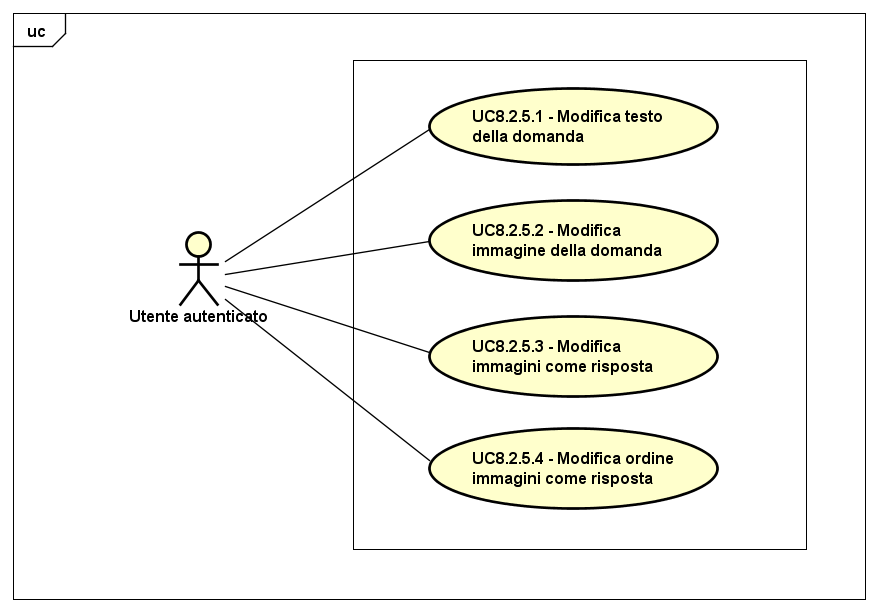
\includegraphics[scale=0.45,keepaspectratio]{UML/UC8_2_5.png}
		\caption{UC8.2.5: Modifica modalità di risposta}
	\end{figure}
	\FloatBarrier
	\begin{itemize}
		\item
			\textbf{Attori}: utente autenticato, utente autenticato pro;
		\item
			\textbf{Scopo e descrizione}: l'utente autenticato modifica la modalità di risposta preferita;
		\item		
			\textbf{Precondizione}: il sistema presenta all'utente autenticato le checkbox per modificare la modalità di risposta;
		\item
			\textbf{Scenario principale}:
	       		\begin{enumerate}
					\item
					L'utente seleziona la modalità di risposta vero o falso [UC8.2.5.1];
					\item
					L'utente seleziona la modalità di risposta a scelta multipla [UC8.2.5.2].
	       		\end{enumerate}
		\item
			\textbf{Postcondizione}: Una modalità di risposta è stata selezionata.
	\end{itemize}
	\subsubsection{Caso d'uso UC8.2.5.1: Selezione modalità di risposta vero o falso}
	\begin{itemize}
		\item
			\textbf{Attori}: Utente autenticato, utente autenticato pro;
		\item
			\textbf{Scopo e descrizione}: L'utente autenticato seleziona la modalità di risposta vero o falso;
		\item		
			\textbf{Precondizione}: Il sistema presenta all'utente autenticato la checkbox per selezionare la modalità di risposta vero o falso;
		\item
			\textbf{Postcondizione}: La modalità di risposta vero o falso è stata selezionata.
	\end{itemize}
	\subsubsection{Caso d'uso UC8.2.5.2: Selezione modalità di risposta a scelta multipla}
	\label{UC8.2.5.2}
	\begin{figure}[h]
		\centering
			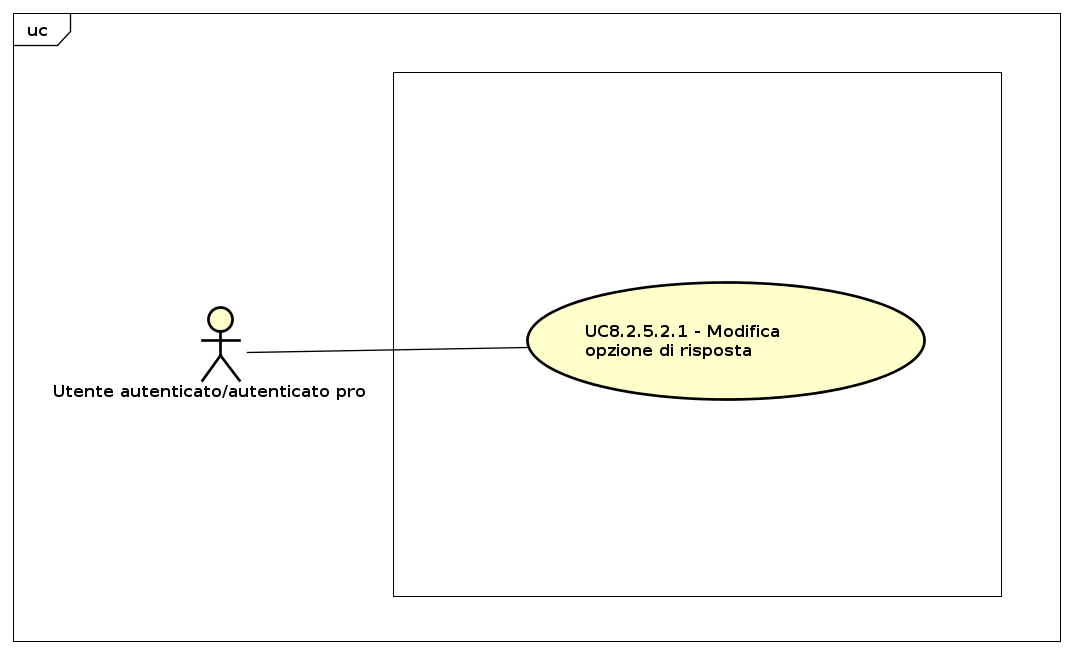
\includegraphics[scale=0.45,keepaspectratio]{UML/UC8_2_5_2.png}
		\caption{UC8.2.5.2: Selezione modalità di risposta a scelta multipla}
	\end{figure}
	\FloatBarrier	
	\begin{itemize}
		\item
			\textbf{Attori}: Utente autenticato, utente autenticato pro;
		\item
			\textbf{Scopo e descrizione}: L'utente autenticato seleziona la modalità di risposta a scelta multipla;
		\item		
			\textbf{Precondizione}: Il sistema presenta all'utente autenticato la checkbox per selezionare la modalità di risposta a scelta multipla;
		\item
			\textbf{Scenario principale}:
				\begin{enumerate}
					\item 	
						L'utente modifica le opzioni di risposta [UC8.2.5.2.1];	
				\end{enumerate}
		\item
			\textbf{Postcondizione}: La modalità di risposta a scelta multipla è stata selezionata.
	\end{itemize}
		\subsubsection{Caso d'uso UC8.2.5.2.1: Modifica opzione di risposta}
		\begin{itemize}
		\item
			\textbf{Attori}: Utente autenticato, utente autenticato pro;
		\item
			\textbf{Scopo e descrizione}: L'utente autenticato modifica le opzioni di risposta della domanda selezionata;
		\item		
			\textbf{Precondizione}: Il sistema presenta all'utente autenticato lo spazio per modificare le opzione di risposta della domanda selezionata;
		\item		
			\textbf{Postcondizione}: L'utente autenticato ha modificato le opzioni di  risposta;
		\end{itemize}
	\subsubsection{Caso d'uso UC8.2.6: Modifica risposta corretta}
		\begin{itemize}
		\item
			\textbf{Attori}: Utente autenticato, utente autenticato pro;
		\item
			\textbf{Scopo e descrizione}: L'utente autenticato modifica la risposta corretta;
		\item		
			\textbf{Precondizione}: Il sistema predispone un strumento per modificare la risposta corretta.
		\item		
			\textbf{Postcondizione}: L'utente autenticato ha modificato la risposta corretta.
		\end{itemize}
